
\section{Results}
\label{sec:results}

The possible plate angles are bounded to be within the range
[-10$^\circ$, +10$^\circ$] with valid variations of $\pm$1$^\circ$:
such constraints are due to the fact that a wider range has a negative impact
on the ball acceleration, making the control more difficult. Moreover, varying
the plate angle beyond $\pm$1$^\circ$ implies an unrefined tuning and a
higher $\dot{\omega}$.

The control period for the simulation, $\Delta t$, is set to 20ms, being a
good trade-off between computational load and the system dynamics.
Longer intervals imply a harder learning because the ball shift widens
causing angle saturations and hence, a greater ball speed.

The plate is square and its side length is 0.40 meters.

The learning phase, reported in Figure~\ref{fig:learning}, took more than 30
hours executing about 27000 simulations.
Each simulation starts placing the ball in a random position on the plate,
initially horizontal, and executes at most $10^6$ learning steps.

\begin{figure}[htb]
  \centering
  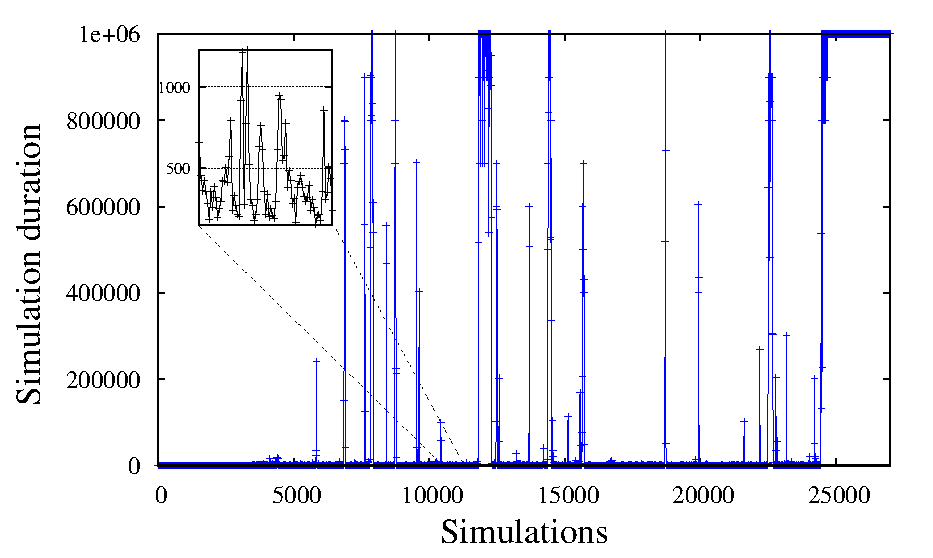
\includegraphics[width=0.9\columnwidth]{result.eps}
  \caption{Learning progress.}
  \label{fig:learning}
\end{figure}

Up to about 24000 simulations, failures occured few steps after the beginning
of the training procedure, except for some sporadic cases in which the ball was
well controlled.
From about 24000 simulations till the training session end (about 27000),
the networks were able to control the ball, keeping always it within the
red boundaries, until the simulation steps limit ($10^6$).

The networks always worked well during the next tests, being able to avoid
failures also when some moderate perturbations were applied through the
graphical program.

% end section

